\documentclass[utf8x,compress,hyperref]{beamer}
\hypersetup{pdfpagemode={FullScreen}}

% \usepackage{graphicx}
% \usepackage[utf8x]{inputenc}
% \usepackage{pgf}
\usepackage{tikz}
% \usetikzlibrary{trees,positioning,arrows}

\usetheme{Malmoe}
\title[Study AFP in SP 3 (Jan-Mar)!]{Why \emph{You} should study\\\href{http://www.student.chalmers.se/sp/course?course_code=TDA342}{Programming Paradigms}}
\author[JP Bernardy, Chalmers and GU]{Jean-Philippe Bernardy, Chalmers and U. of Gothenburg}
% ate{2010-11-16}
\begin{document}
\section{Programming Paradigms}
\subsection{Summary}
\begin{frame}
\maketitle
Paradigm = School of Thought
\begin{itemize}
\item Philosophy --- Learn new ways to think! (your programs)
\item Competitive advantage --- Knowing a paradigm can be the
  difference between success and failure of a project. \\
If you don't know how how to structure your thoughts, you may get
bogged down in implementation details.
\end{itemize}

\end{frame}

\subsection{Context}
\begin{frame}

Basic buiding block for the ``programming-languages'' track:

\hspace{2cm}
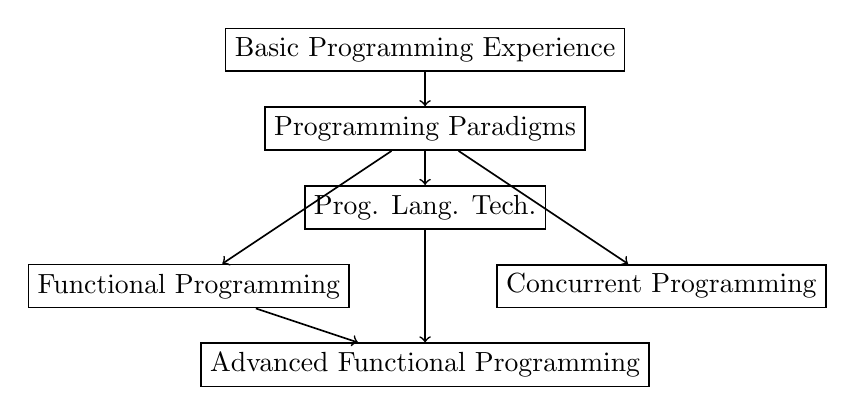
\begin{tikzpicture}[line width = 0.6pt]
\tikzstyle{every node}=[rectangle,draw];
   
\draw(0,4) node (Base) {Basic Programming Experience};
\draw(0,3) node (PP) {Programming Paradigms};
\draw(3,1) node (CP) {Concurrent Programming};
\draw(-3,1) node (FP) {Functional Programming};
\draw(0,2) node (Prog) {Prog. Lang. Tech.};
% \draw(0,2) node (LiCS) {Logic in CS};
\draw(0,0) node (AFP) {Advanced Functional Programming};

\draw[->] (Base) -- (PP);
\draw[->] (PP) -- (FP);
\draw[->] (PP) -- (Prog);
\draw[->] (PP) -- (CP);
\draw[->] (FP) -- (AFP);
% \draw[->] (LiCS) -- (AFP);
\draw[->] (Prog) -- (AFP);
\end{tikzpicture}

\begin{itemize}
\item Chalmers+GU is strong in programming language research.
\item All the above courses (and others in the same track) are given
  by world-class researchers in the domain.
\item Programming Paradigms = excellent starting point on that track
\end{itemize}

\end{frame}

\subsection{Contents}
\begin{frame}
Basic experience of each of the following paradigms:
  \begin{itemize}
  \item Imperative 
  \item Object-Oriented
  \item Functional
  \item Concurrent
  \item Logic
  \end{itemize}

 How to translate between each paradigm:

\fbox{
    think in any paradigm + code in any language 
    = fluidity
}
\pause 

\begin{itemize}
\item Self-study
\item Lectures
\item Exercises
\end{itemize}

\end{frame}


\begin{frame}

\textbf{Learning Outcomes}

\scriptsize
Knowledge and understanding
\begin{itemize}
\item Explain and contrast the principles of different paradigms both
conceptually and in terms of particular language features.
\item Know the relationship between mainstream programming languages, the
features they implement, and the paradigms they support.
\end{itemize}


Skills and abilities

\begin{itemize}
\item Write small idiomatic programs in languages that represent
  different paradigms.

\item Read programs written idiomatically in a given paradigm, and
  translate (encode) them into a language that does not support the
  paradigm directly.

\item Read non-idiomatic programs (that use an encoding), and re-write
  them in their idiomatic paradigm.
\end{itemize}


Judgement and approach
\begin{itemize}
\item 
  Evaluate and apply the styles and strategies that characterize
  different paradigm and assess their suitability for solving a given
  problem.

\item 
  Recognize the paradigms underlying any given program's design,
  regardless of shallow implementation choices.
\end{itemize}
\end{frame}

\end{document}
